\part{Results}
\chapter{Ewald Embedded Cluster}
\label{chap:jctc}
This chapter is adapted from the published version of Reference \citenum{Rivera2019}.

\begin{figure}[h]
\centering
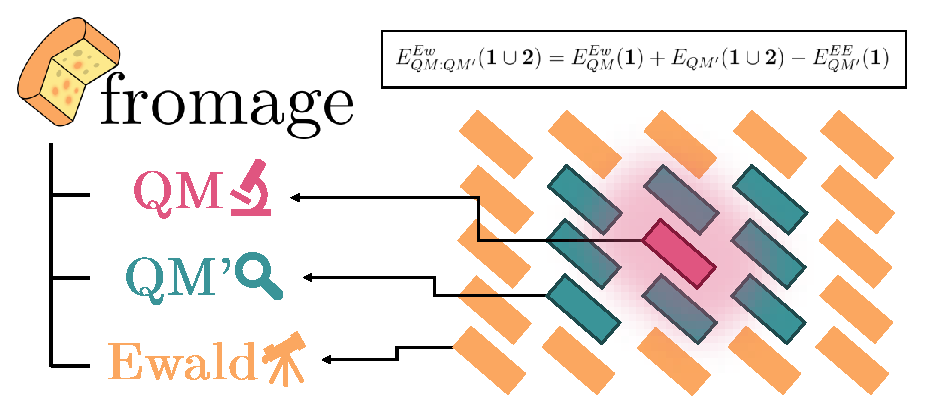
\includegraphics[width=8cm]{Chapters/5Ewald/TOC.pdf}

\label{fig:toc_jctc}
\end{figure}


% \section{Abstract}

% Understanding photoinduced processes in molecular crystals is central to the design of highly emissive materials such as organic lasers and organic light-emitting diodes. The modelling of such processes is, however, hindered by the lack of excited state methodologies tailored for these systems. Embedding approaches based on the Ewald sum can be used in conjunction with excited state electronic structure methods to model the localised excitations which characterise these materials. In this article, we describe the implementation of a two-level ONIOM(QM:QM') point charge embedding approach based on the Ewald method, the ONIOM Ewald Embedded Cluster (\EEC{}) model. An alternative self-consistent method is also considered to simulate the response of the environment to the excitation. Two molecular crystals with opposing photochemical behaviour were used to benchmark the results with single reference and multireference methods. We observed that the inclusion of an explicit ground state cluster surrounding the QM region was imperative for the exploration of the excited state potential energy surfaces. Using \EEC{}, accurate absorption and emission energies as well as S$_1$\textendash{}S$_0$ conical intersections were obtained for both crystals. We discuss the implications of the use of these embedding schemes considering the degree of localisation of the excitation. The methods discussed herein are implemented in an open source platform (\texttt{fromage}, \href{https://github.com/Crespo-Otero-group/fromage}{https://github.com/Crespo-Otero-group/fromage}) which acts as an interface between popular electronic structure codes (\texttt{Gaussian}, \texttt{Turbomole} and \texttt{Molcas}). 

\section{Introduction}


% Highly emissive organic crystals have great potential for the development of optoelectronic and photonic devices such as organic-light-emitting diodes and organic lasers.\cite{Li2014a,Lee2015,Gierschner2016} The electronic structure of the constituent monomers, intermolecular interactions and the electrostatic field in the crystal environment all contribute to the competition between radiative and nonradiative pathways, such as internal conversion and intersystem crossing. The exploration of excited state potential energy surfaces (PESs) in the solid state can help decipher the role of these interconnected factors and rationalise observed quantum yields. 


Excitations in organic molecular crystals have been found to localise on only a few constituent monomers of the crystal.\cite{Arag2015} This poses a challenge for traditional electronic structure methods, which have been designed to describe either highly localised or periodic delocalised electronic states. In this context, embedding techniques, such as those discussed in Chapter \ref{chap:emb}, represent a viable option by combining higher quantum mechanical levels of theory to describe the excited region (QM) and more approximate methods for the crystal environment (QM' or MM).\cite{SeveroPereiraGomes2012a} 

Within the ONIOM scheme, the QM' method can be chosen to be plane-wave DFT\cite{Kochman2013,Kochman2013a} for a natural description of the lattice periodicity, although this usually means sacrificing the electrostatic embedding. Correlated wavefunction-in-DFT periodic embedding approaches are a promising alternative\cite{Libisch2014,Cheng2017,Cheng2017a}. One of the most common approaches is to use cluster models to describe the periodic crystal.\cite{Presti2014,Presti2016a,Presti2016} The cluster is extracted from the atomic lattice positions and provides an energetic description of the short-range interactions with the QM region.

In the case of ionic or highly polar crystals, long-range interactions can be of great importance since the electrostatic potential is slowly and conditionally convergent. This prompts the use of the Ewald summation, to evaluate long-range Coulomb interactions in the crystal (see Section \ref{sec:ewald}).

When considering embedded finite cluster models, the electrostatic embedding can be modified to reflect the Ewald potential. In this case, the electrostatic interactions affecting the QM region extend beyond just the short-range and up to the infinitely large in a periodic system. Klintenberg \textit{et al.} developed a methodology where a large array of point charges is fitted to reproduce the exact Ewald potential inside the QM region of a cluster model.\cite{Klintenberg2000,Derenzo2000,Weber2010} This procedure has been used for the investigation of ionic crystals and the calculation of NMR parameters in organic crystals.\cite{Jug2004,Weber2010,Stueber2001} Sokol \textit{et al.} have implemented a related method in Chemshell to model defects in ionic materials.\cite{Sokol2004,Metz2014} An alternative is the procedure proposed by Abrenkov and Sushko, where compensating point charges are added within unit cells to approach the Ewald potential.\cite{Abarenkov2007,Sushko2010}   

Ewald embedding methods have been used with QM:MM and ONIOM approaches allowing the evaluation of the short-range non-Coulombic interactions.\cite{Kobayashi2015a,Nam2005a,Wang2013a,Sushko2013a,Sousa2013a,Cui2011a} However a simpler variant is the Point Charge Embedding approach (PCE) where only the Coulomb interactions are considered, using point charges, and non-electrostatic interactions are neglected.\cite{SeveroPereiraGomes2012a,Weber2010} The performance of these  methods for the investigation of excited states PESs of molecular crystals is relatively unexplored. Recently, Ciofini and co-workers\cite{Wilbraham2016a,Presti2017,Wilbraham2018} have implemented an Ewald PCE scheme based on the method proposed by Derenzo \textit{et al.}.\cite{Derenzo2000} In order to consider mutual polarisation effects of the crystal environment, a self-consistent algorithm was employed in the investigation of a crystal displaying aggregation-induced emission.\cite{Presti2017} Self-consistent schemes are typical tools used in QM:MM schemes when the polarisation of the environment is important.\cite{Cieplak2009,Warshel2007,Xie2007}

In this chapter, we present different Ewald embedding approaches for the description of PESs of molecular crystals, with specific focus on the treatment of excited state minima and conical intersections. We show that due to the lack of short-range non-Coulombic interactions, geometry optimisation with the PCE method can be extremely problematic. As a solution, we implement an Ewald-embedded QM:QM' cluster model that can be used to explore the PES of flexible molecules. We assess the efficacy of these schemes with two crystals based on 2'-hydroxychalcone (\HC{} and \HCC{}, shown in Figure \ref{fig:molecules}). These molecules undergo excited state intramolecular proton transfer (ESIPT), where the large changes in electronic structure in the excited state pose a challenge to embedding methods. The figure represents the enol (\textbf{E}) form. The keto form (\textbf{K}), where the proton is bonded to the other oxygen atom, is unstable in the ground state.

\begin{figure}
\centering
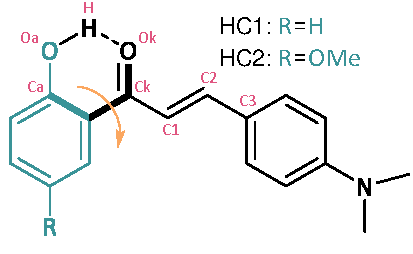
\includegraphics[width=7cm]{Chapters/5Ewald/molecules.pdf}
\caption{Molecular diagram of the 2’-hydroxychalcone derivatives, \HC{} and \HCC{}. The access to conical intersections for theses molecules is centred around the rotation of the blue group about the dihedral angle shown in bold. The notable atoms with large partial charge are labelled in pink.}
\label{fig:molecules}
\end{figure}

Our group has previously investigated \textbf{HC1} and \textbf{HC2} in the context of Solid State Luminescent Enhancement (SSLE).\cite{Dommett2017a,Dommett2017c} We opt for the term SSLE over Aggregation Induced Emission (AIE), which is more popular in the field, because it is more specific, as outlined in Reference \citenum{Shi2017}.
The population of the keto (\textbf{K*}) and enol (\textbf{E*}) excited states depends on the identity of the substituents and crystal packing.\cite{Dommett2017c} \HC{} displays emission in the crystal with promising properties to be used in solid state lasers\cite{Zhang2015} and predominantly forms herringbone-type aggregates. In contrast, \HCC{}'s decay is mainly non-radiative and its crystal structure features mainly $\pi$-stack dimers. Their excited state PESs were found to be particularly sensitive to the electrostatic environment. The SLE character of \HC{} can be understood using the Restricted Access to Conical Intersections (RACI) model\cite{Blancafort2018,Li2013a} wherein upon aggregation the energy of the S$_1$-S$_0$ conical intersections increases, thereby blocking nonradiative deactivation pathways and enhancing the emissive response.

The chapter is organised as followed. First, we present the different embedding models and the details of their implementation. Next, we define how to choose the size of the high-level QM region, an important step in the division of the cluster regions. We then determine the effect of different point charge embedding schemes and assess their overall performance. In our conclusions, we suggest a protocol for researchers studying excited states in molecular crystals. The presented methodologies are implemented in a new open-source platform: \texttt{fromage} (FRamewOrk for Molecular AGgregate Excitations). 


\section{Embedding Schemes}
\label{sec:theo}
\subsection{Point Charge Embedding}
We consider two electrostatic Ewald embedding approaches to investigate excited states in molecular crystals: PCE and a two-level ONIOM(QM:QM') model. For the PCE approach, where only the Coulombic interactions are considered, we adopt a strategy similar to that proposed by Wilbraham \textit{et al.}\cite{Wilbraham2016a}. The atomic charges were obtained using the \texttt{Ewald} program from Derenzo \textit{et al.} \cite{Derenzo2000} after being modified to allow non-integer charge values. The origin of the charges is discussed in Section \ref{sec:origin_charges}. The effect of the polarisation of the environment was considered for both methods within a self-consistent embedding algorithm. These approaches were implemented in \texttt{fromage}, the source code and the documentation are available online.\cite{fromage,fromagedoc}

In the \texttt{Ewald} program,\cite{Derenzo2000} an array of about $10^{4}$ charges is generated from a supercell. Three zones are defined, the central region (zone \textbf{I}) is where the highest level of theory will be used. It is spherically surrounded by a buffer region (zone \textbf{II}) of approximately 500 point charges. Charges of both zone \textbf{I} and \textbf{II} are held constant. The rest of the charges (zone \textbf{III}) are altered to reproduce the Ewald potential in the central and buffer regions upon the direct summation of all point charges. The algorithm removes any artificial dipole moment introduced in the procedure. A detailed description of the method and the corresponding program can be found in Reference \citenum{Derenzo2000}.

The implementation of PCE in \texttt{fromage} consists of electronic structure calculations at zone \textbf{I} atomic sites, embedded in the atomic charges of zones \textbf{II} and \textbf{III}. For clarity, we refer to zone \textbf{II} and \textbf{III} charges as Ewald charges. Excited state energies are obtained with TDDFT, CASSCF, CASPT2 and CC2 \textit{via} interfaces with \texttt{Gaussian},\cite{g16} \texttt{Molcas},\cite{Aquilante2016} and \texttt{Turbomole}\cite{TURBOMOLE}. An interface with \texttt{DFTB+}\cite{Aradi2007} is under development. The atomic charges can be obtained from molecular or periodic crystal calculations. We consider RESP, Mulliken and NBO from molecular calculations and RESP, Mulliken, Hirshfeld and AIM charges from periodic calculations. Currently, atomic charges can be read from \texttt{Gaussian} and \texttt{CP2K}.
  
 \texttt{fromage} provides tools for the exploration of PESs of molecular crystals. The L-BFGS minimisation algorithm is used to locate stationary points. A complete characterisation of excited state potential energy surfaces in molecular crystals require the description of conical intersections. We have implemented the penalty function method of Levine \textit{et al.}\cite{Levine2008} to optimise Minimal Energy Conical Intersection (MECI) geometries. In contrast with other methods,\cite{Ruiz2015} this approach does not require nonadiabatic coupling vectors. A function of the averaged S$_1$ and S$_0$ energies ($\bar{E}_{1-0}$) and the S$_1$\textendash{}S$_0$ energy gap ($\Delta E$) is minimised:
\begin{equation}
\label{eq:ciopt}
F = \bar{E}_{1-0} + \sigma \frac{\Delta E^2}{|\Delta E|+ \alpha}
\end{equation}
where $\sigma$ is a Lagrangian multiplier and $\alpha$ is a parameter such that $\alpha \ll |\Delta E|$. The purpose of this functional form is to find a smooth minimum for the S$_1$\textendash{}S$_0$ energy difference, with a weight $\sigma$, whilst minimising the overall energy with a weight $1/\sigma$.

This algorithm is implemented in \texttt{fromage} for CASSCF, CC2 and TDDFT electronic methods. We would like to emphasise that even when multireference quantum methods are preferable for modelling S$_1$\textendash{}S$_0$ crossings,\cite{Levine2007,Barbatti2014} in many cases single-reference methods can provide a qualitative description of these regions of the PES. Conical intersections can approximatively be described with single-reference methods such as TDDFT.\cite{Barbatti2014} Nonadiabatic dynamics simulations with these methods have shown for multiple systems that methods such as ADC(2) and CC2 can provide reasonable results.\cite{Gozem2014a,Tuna2015} In the case of TDDFT, a careful selection of the functional is required.\cite{Crespo-Otero2014,Barbatti2015} Considering the computational cost of multireference methods and the sensitivity of their active space, it can at times be necessary to resort to single-reference methods. However, their performance near S$_1$\textendash{}S$_0$ crossings should be carefully tested by comparison with multireference calculations.




\subsection{Ewald Embedded ONIOM QM:QM'}
\label{sec:oniom_energy}

Geometry optimisation and conical intersection search become problematic within the PCE scheme because of the lack of short-range non-Coulombic interactions which results in overpolarisation effects (see section \ref{sec:PCE}). To overcome these limitations, we formulate an ONIOM\cite{Chung2015} Ewald Embedded Cluster (\EEC{}) model. It is devised as an extension of the commonly used ONIOM Embedded Cluster model (\EC{}) which usually only includes electrostatic embedding up to the range of the cluster. We consider a QM:QM' scheme rather than QM:MM to avoid the need for specific parameterisation.

We wish to expand upon the electrostatically embedded expression for the ONIOM QM:QM' energy discussed in Chapter \ref{chap:emb} by including long-range electrostatic effects. To do so, we begin by deriving the ONIOM equation. To define a total energy expression, we state the energy of the whole crystal divided into regions \textbf{1}, \textbf{2} and \textbf{3}, where \textbf{3} surrounds \textbf{2} which surrounds \textbf{1}. Regions \textbf{2} and \textbf{3} will be fixed in place whereas region \textbf{1} is allowed to reorganise. We denote inter-region interactions as $E^{\text{int}}(\bm{i} \cup \bm{j})$ which can be split between electrostatic ($E^{\text{ES}}(\bm{i} \cup \bm{j})$) and other ($E^{\text{X}}(\bm{i} \cup \bm{j})$) interactions.

\begin{equation}
\begin{split}
E(\bm{1} \cup \bm{2} \cup \bm{3}) = &E(\bm{1}) + E(\bm{2}) + E(\bm{3}) + E^{\text{int}}(\bm{1} \cup \bm{2}) + E^{\text{int}}(\bm{1} \cup \bm{3}) + E^{\text{int}}(\bm{2} \cup \bm{3}) + E^{\text{int}}(\bm{1} \cup \bm{2} \cup \bm{3})\\
 = &E(\bm{1}) + E(\bm{2}) + E^{\text{int}}(\bm{1} \cup \bm{2}) + E^{\text{int}}(\bm{1} \cup \bm{3}) + E^{\text{int}}(\bm{1} \cup \bm{2} \cup \bm{3}) + \text{const.}\\
 = &E(\bm{1}) + E(\bm{2}) + E^{\text{ES}}(\bm{1} \cup \bm{2}) + E^{\text{X}}(\bm{1} \cup \bm{2}) + E^{\text{ES}}(\bm{1} \cup \bm{3}) + E^{\text{X}}(\bm{1} \cup \bm{3}) + E^{\text{int}}(\bm{1} \cup \bm{2} \cup \bm{3})\\
 &+ \text{const.}
\end{split}
\label{eq:full_ener}
\end{equation}

We can neglect the $E^{\text{X}}(\bm{1} \cup \bm{3})$ term since Coulombic interactions dominate the long range regime. The nonadditive three-body term $E^{\text{int}}(\bm{1} \cup \bm{2} \cup \bm{3})$ is also neglected in this picture, as the freezing of $\bm{2}$ and $\bm{3}$ should drive it down significantly, and we wish to avoid modelling infinitely many molecules. By further removing the constant, and assigning different levels of theory to the various terms, we obtain an expression for the hybrid QM:QM' energy:

\begin{equation}
\tilde{E}^{\text{OEEC}}_{\text{QM}:\text{QM}'}(\bm{1} \cup \bm{2}) = \big [ E_{\text{QM}}(\bm{1}) + E_{\text{QM}}^{\text{ES}}(\bm{1} \cup \bm{2}) + E_{\text{QM}}^{\text{ES}}(\bm{1} \cup \bm{3}) \big ] + \big [ E_{\text{QM}'}(\bm{2}) + E_{\text{QM}'}^{\text{X}}(\bm{1} \cup \bm{2}) \big ]\\
\label{eq:tilde}
\end{equation}

Here, the first bracket can be approximated via a QM level calculation of the region $\bm{1}$ energy, electrostatic embedded with whichever point charges will best represent the electrostatic interactions between $\bm{1}$ and $\bm{2} \cup \bm{3}$. We use the notation:


\begin{equation}
E_{\text{QM}}(\bm{1}) + E_{\text{QM}}^{\text{ES}}(\bm{1} \cup \bm{2}) + E_{\text{QM}}^{\text{ES}}(\bm{1} \cup \bm{3}) \approx E_{\text{QM}}^{\text{Ew}}(\bm{1})
\label{eq:mhemb}
\end{equation}

For the second bracket, we can use a similar strategy:

\begin{equation}
\begin{split}
E_{\text{QM}'}(\bm{2}) + E_{\text{QM}'}^{\text{X}}(\bm{1} \cup \bm{2}) & = E_{\text{QM}'}(\bm{1} \cup \bm{2}) - E_{\text{QM}'}(\bm{1}) - E_{\text{QM}'}^{\text{ES}}(\bm{1} \cup \bm{2})\\
& \approx E_{\text{QM}'}(\bm{1} \cup \bm{2}) - E_{\text{QM}'}^{\text{EE}}(\bm{1})
\end{split}
\label{eq:mlemb}
\end{equation}

Where $E_{\text{QM}'}^{\text{EE}}(\bm{1})$ denotes an energy calculation of region $\bm{1}$ embedded in QM' charges from region $\bm{2}$. We embed in QM' charges since the role of the embedding is to reflect the electrostatic interactions between regions $\bm{1}$ and $\bm{2}$ at the QM' level of theory.

By inserting approximations \ref{eq:mhemb} and \ref{eq:mlemb} in to equation \ref{eq:tilde}, we obtain a total energy expression:

\begin{equation}
E_{\text{QM}:\text{QM}'}^{\text{OEEC}}(\bm{1} \cup \bm{2}) = E_{\text{QM}}^{\text{Ew}}(\bm{1}) + E_{\text{QM}'}(\bm{1} \cup \bm{2}) - E_{\text{QM}'}^{\text{EE}}(\bm{1})
\label{eq:ener_sup}
\end{equation}
The hybrid gradients are defined accordingly.

To relate this equation to molecular clusters, a graphical representation of our \EEC{} model is shown in Figure \ref{fig:maineq}. The \EEC{} model is comprised of two regions, the central region \textbf{1} (corresponding to zone \textbf{I} in the \texttt{Ewald} program) and nearest-neighbour molecules (\textbf{2}). Region \textbf{2} should be large enough to include the most important short-range non-electrostatic interactions with the QM cluster. The buffer region defined for \texttt{Ewald} (zone \textbf{II}) does not necessarily correspond to region \textbf{2}.

\begin{figure}
    \centering
    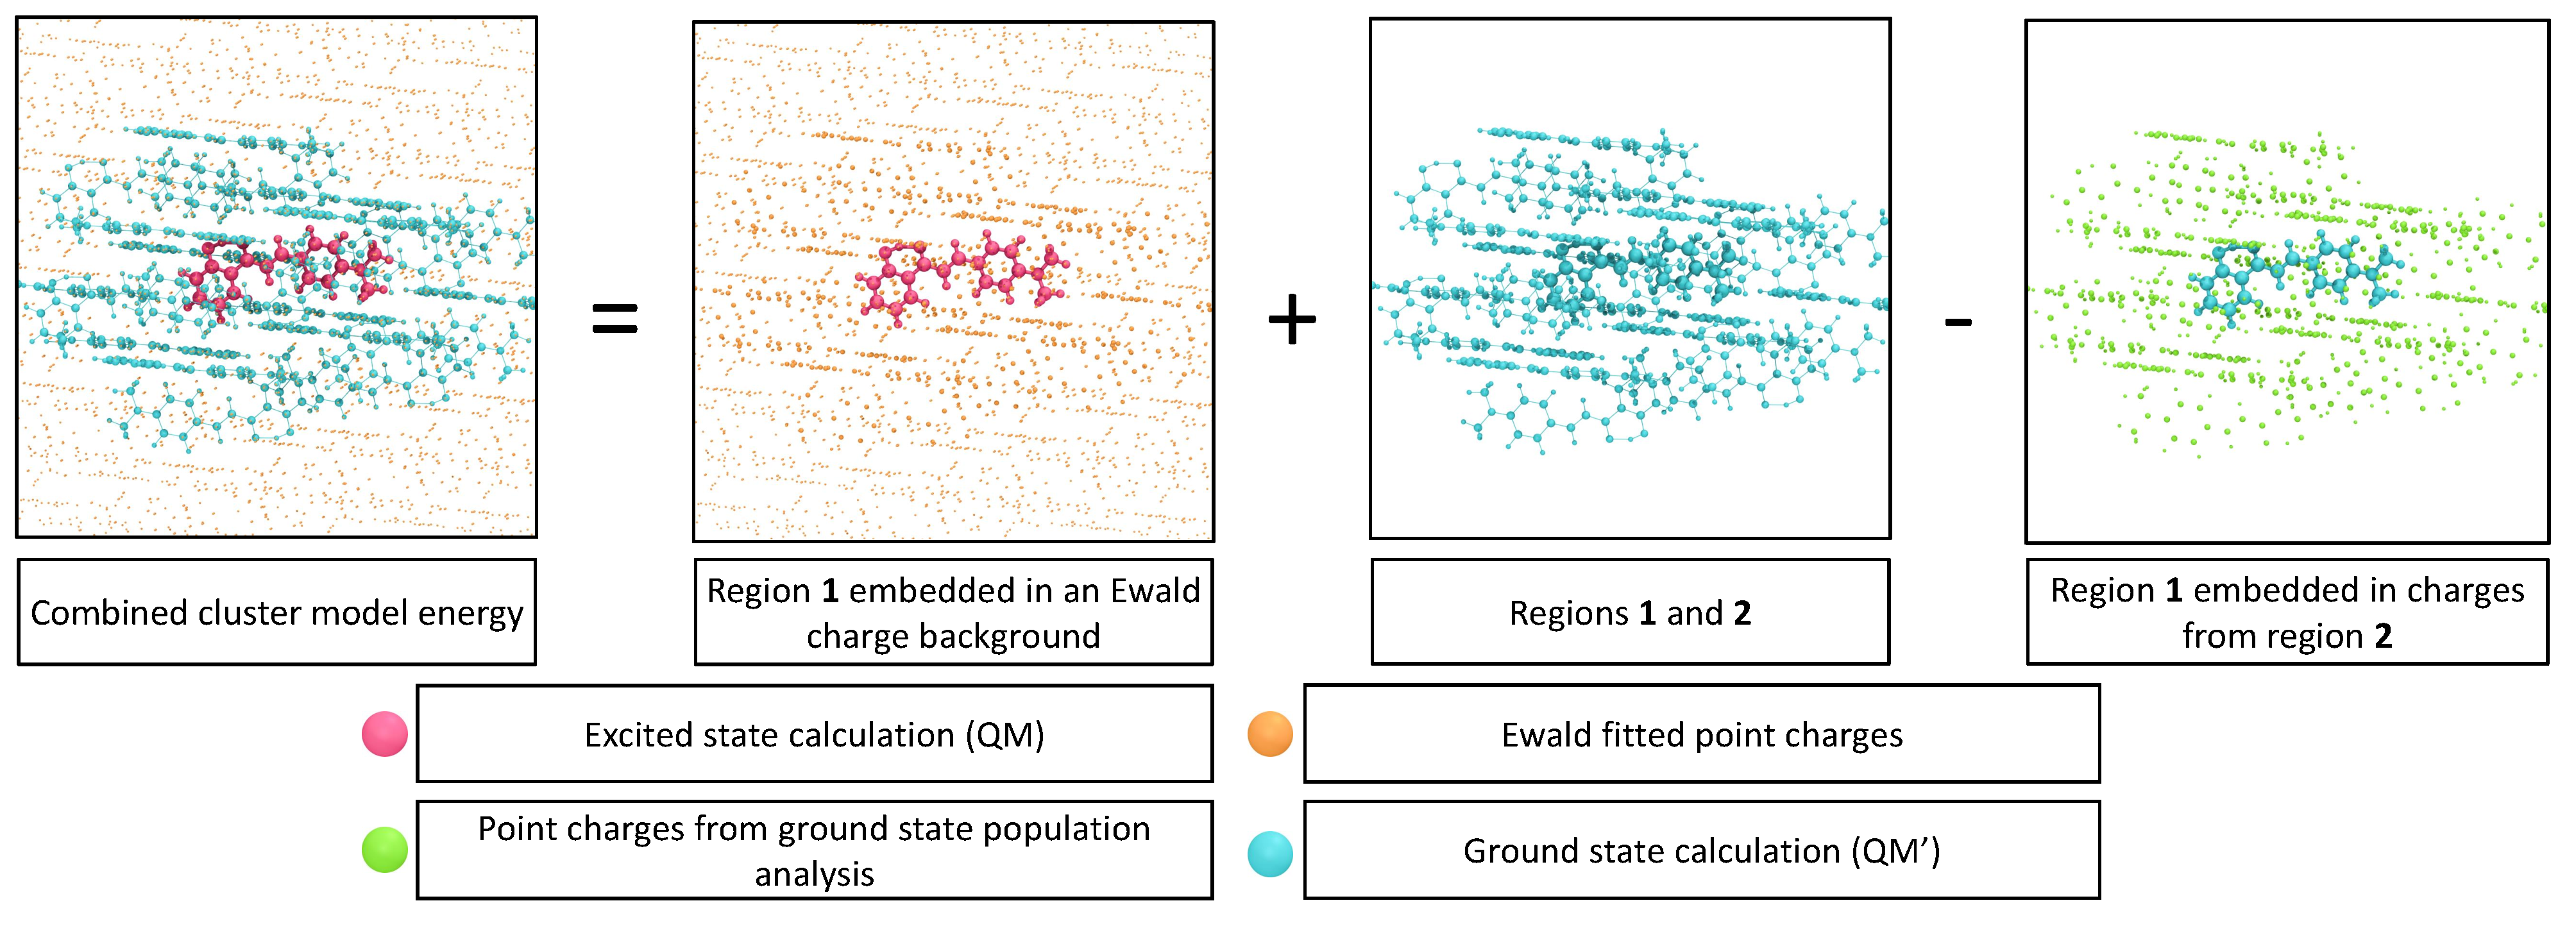
\includegraphics[width=17cm]{Chapters/5Ewald/main_eq.pdf}
    \caption{Visual representation of the main energy equation for the Ewald Embedde Cluster model.}
    \label{fig:maineq}
\end{figure}

In the \EEC{} scheme, Coulombic interactions of any distance between region \textbf{1} and the crystal are described at the higher level of theory (QM). For excited state calculations, this represents the interaction between an excited central region and the environment in the ground state, unless particular charges are considered in the \texttt{Ewald} algorithm (\textit{vide infra}). In contrast, the short-range non-Coulombic interactions between \textbf{1} and \textbf{2} are considered at the QM' ground state level, which recovers some of the short-range contributions and improves the description provided by PCE. Since non-Coulombic interactions are considered in the ground state, for fixed geometries the energy gaps are equivalent to those obtained with the PCE. The selection of the QM' level of theory depends on the available computational resources. Previous studies on truncated cluster models have shown that low levels of theory such as HF/STO-3G achieve accurate results.\cite{Kochman2013,Wilbraham2016a,Presti2016a,Presti2016,Presti2017}


In order to consider the response of the environment to the excitation and recover mutual polarisation effects, we employ the extension of self-consistent Ewald embedding to excited states proposed by Wilbraham \textit{et al.}\cite{Wilbraham2016a}. Mutually polarising embedding methods have been applied to a number of ground state systems.\cite{Kepenekian2009,Stueber2001,Guennic2007,Weber2010} In the self-consistent approach, a QM-level calculation is carried out on a quantum cluster. A population analysis is then applied and the charge values are re-assigned to the equivalent positions in the crystal. Those charges are then fitted using \texttt{Ewald} and another QM calculation is carried out. The loop between Ewald fitting and population analysis is repeated until convergence of the atomic charges. The new charge background is used for the electrostatic embedding of \textbf{1}. In \texttt{fromage}, the self-consistent approach is implemented for the PCE and the QM/QM' approaches (SC-PCE and SC-\EEC{}). We consider two versions which may represent different physical situations in the crystal (discussed in section \ref{sec:loc}). The first, SC-PCE-S$_1$, closely corresponds to the embedding proposed by Wilbraham \textit{et al.}; it uses excited state charges as an initial charge background and iterates with excited state population analyses. The second, SC-PCE-S$_0$, has a ground state initial charge background and performs ground state population analyses. We extend these methods to SC-OEEC-S$_1$ and SC-OEEC-S$_0$. For ease of reading, the embedding models are listed in Table \ref{tab:acro}. Note that it is impossible to provide a self-consistent charge environment where the central molecule is in the excited state and the surrounding ones are in the ground state, if we are to preserve the periodicity of the Ewald method.

\begin{table}
\centering
\caption{Embedding models used in this study}
\label{tab:acro}
\def\arraystretch{1.5}
\begin{tabular}{cm{6cm}m{6cm}}
\toprule
\textbf{Acronym} & \textbf{Full name} & \textbf{Description}\\\midrule
PCE & Point Charge Embedding & Point charge embedding fitted to match the Ewald potential \\\hdashline
SC-PCE-S$_1$ & Self-Consistent Point Charge Embedding & PCE computed self consistently in S$_1$\\\hdashline
SC-PCE-S$_0$ & Self-Consistent Point Charge Embedding & PCE computed self consistently in S$_0$\\\hdashline
\EC{} & ONIOM Embedded Cluster & QM:QM' ONIOM cluster model with the QM region embedded in charges from the QM' region\\\hdashline
\EEC{} & ONIOM Ewald Embedded Cluster & \EC{} with the QM region embedded in charges from PCE\\\hdashline
\SCEEC{}-S$_1$ & Self-Consistent ONIOM Ewald Embedded Cluster S$_1$ & \EC{} with the QM region embedded in charges from SC-PCE-S$_1$\\\hdashline
\SCEEC{}-S$_0$ & Self-Consistent ONIOM Ewald Embedded Cluster S$_0$ & \EC{} with the QM region embedded in charges from SC-PCE-S$_0$\\\bottomrule
\end{tabular}

\end{table}

For SC-PCE-S$_1$, the convergence of the charge values can be sped up by starting the loop from a ground state population analysis embedded in ground state Ewald charges. The final background was found to be very similar, with an RMSD of $10^{-5}$ $\mathrm{e^-}$ for atomic charges. Another alternative is to perform the loop on a molecule which has already been optimised in the excited state using \EEC{}. In this case, the equilibration of the charge background is made to match the excited state minimum, however this implies assigning charges from an excited state minimum configuration to region \textbf{2} molecules which are in their ground state minimum geometry.




Figure \ref{fig:sc} describes the structure of \texttt{fromage}. The charge background can be chosen to be computed self-consistently and the geometry optimisation can be set to search for ground and excited state minima or MECI. Currently, region \textbf{2} is fixed in place during geometry optimisation, although full cluster relaxation\cite{Ruiz2015} is under development. For \SCEEC{}, to recover point charges of the highest quality, the molecule of interest in the unit cell is first relaxed with \EEC{}. Furthermore the self-consistent charge background is computed only for the first step, at the ground state \EEC{} geometry, in order to maintain a consistent PES throughout the relaxation.

\begin{figure}
\centering
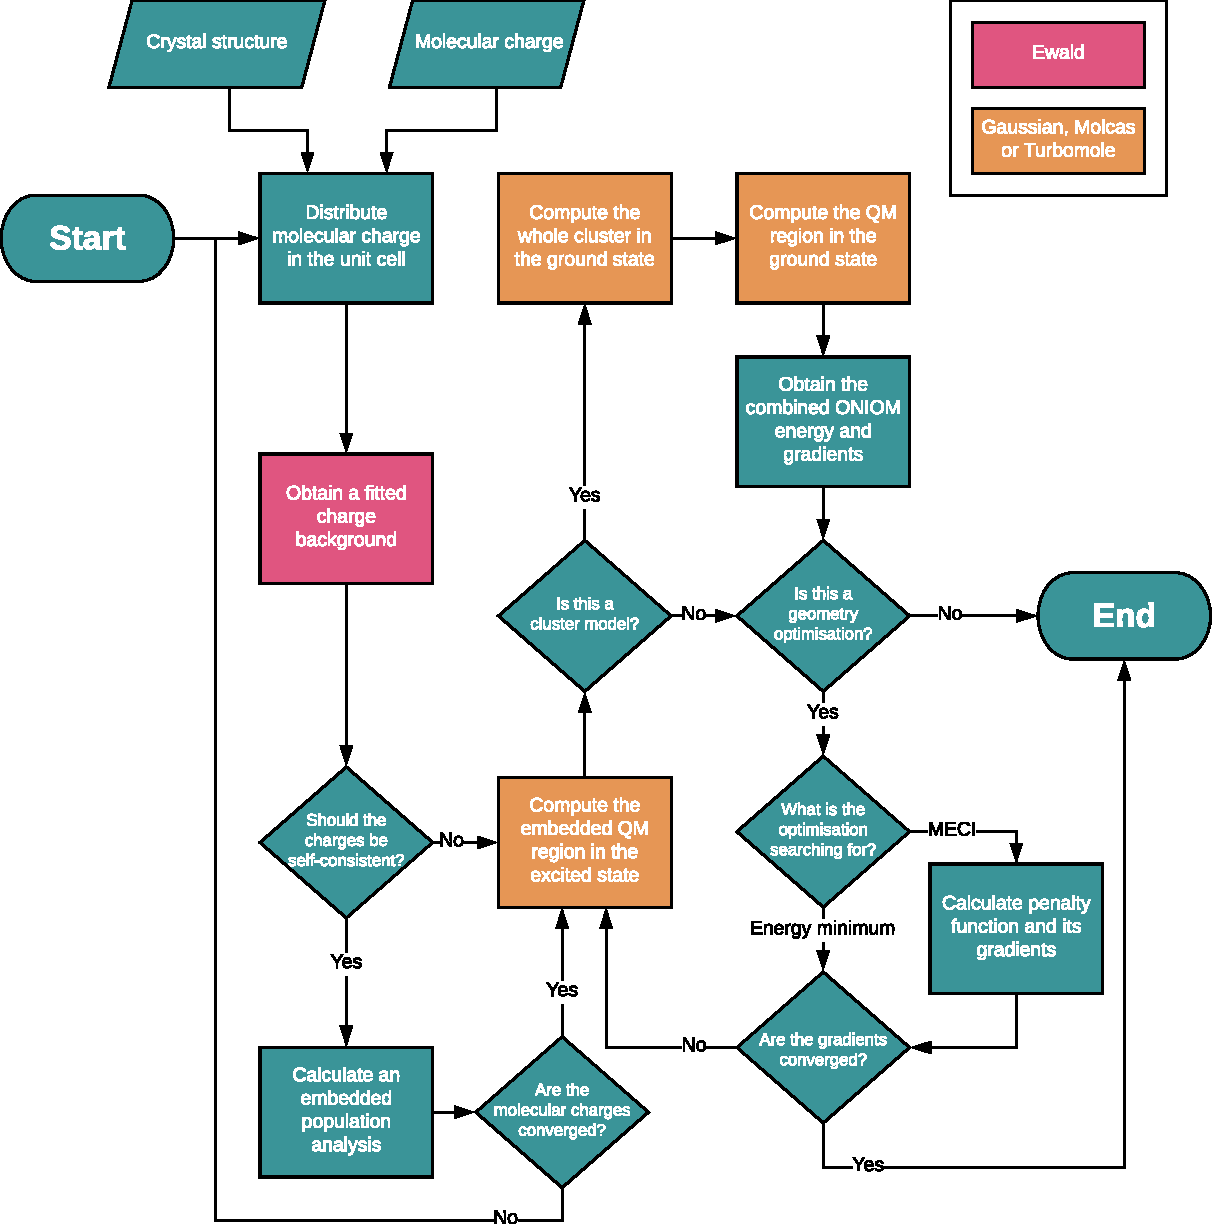
\includegraphics[width=14cm]{Chapters/5Ewald/sc_diagram2.pdf}
\caption{Flowchart of a calculation using the ONIOM Ewald Embedded Cluster (\EEC{}) and Self-Consistent ONIOM Ewald Embedded Cluster (\SCEEC{}) models. The electronic program can be chosen by the user.}
\label{fig:sc}
\end{figure}

\subsection{Origin of Point charges}
\label{sec:origin_charges}
The usual electrostatically embedded QM:QM' ONIOM model has the following energy expression:
\begin{equation}
E_{\text{QM}:\text{QM}'}^{\text{EE}}(\bm{1} \cup \bm{2}) = E_{\text{QM}}^{\text{EE}}(\bm{1}) + E_{\text{QM}'}(\bm{1} \cup \bm{2}) - E_{\text{QM}'}^{\text{EE}}(\bm{1})
\label{eq:ener_sup_trad}
\end{equation}


Traditional implementations use charges originating from QM' calculations in the embedding of the QM calculation in order to mitigate the overpolarisation arising when the QM wavefunction approaches the singular potential well of the point charge.\cite{Hratchian2008} The objective is to cancel out errors arising from the point charge approximation in the short range in the first and third terms of equation \ref{eq:ener_sup_trad}. However this cancellation becomes less exact when the region \textbf{1} QM charge density differs significantly from the QM' charge density as is the case when considering excited states. Furthermore, usual ONIOM schemes are designed to account for inter-region boundaries crossing a bond (and using link atoms to correct the dangling bond). In the cases discussed herein, the region boundary is defined inter- rather than intramolecularly and most intermolecular contacts are larger than 4 \r{A}, making the usual choice of point charge less pertinent.

Moreover, in traditional ONIOM QM:QM', assuming a well behaved cancellation of point charge overpolarisation, the electrostatic potential of region \textbf{2} on \textbf{1} stems entirely from the $E_{\text{QM}'}(\bm{1} \cup \bm{2})$ term, thus causing the choice of point charges in the embeddings of $E_{\text{QM}}^{\text{EE}}(\bm{1})$ and $E_{\text{QM}'}^{\text{EE}}(\bm{1})$ to be of little overall impact as long as they match. In contrast, equation \ref{eq:ener_sup} aims to cancel out the potential between the second and third term, thus relying entirely on the embedding of the first term for a high quality electrostatic potential of regions $\bm{2}$ and $\bm{3}$ on $\bm{1}$.

Therefore in the implementation discussed herein, we principally use ground state QM charges in the embedding of the first term and ground state QM' charges for the final term. However, all other embedding combinations are available in \texttt{fromage}. Further extensions of these methods can be implemented to reduce artificial polarisation\cite{Biancardi2016} and make the methods useful for more dense systems.

The alternative scheme where Ewald charges are used for the QM' calculations should provide a marginally worse compensation of the inter-region Coulombic interactions. Nevertheless, the results obtained with this embedding scheme are similar to those obtained with the cluster charges for \HC{}. The absorption energies are only deviated by 0.01 eV from those obtained with the original scheme. In the case of the emission energies from the \textbf{K} form, the value obtained with this version of \EEC{} is 2.24 eV which is in relative good agreement with the results obtained with other schemes (Table \ref{tab:em_abs}). Indeed by extending the QM' point charges to into region $\bm{3}$ the only non-constant term which is artificially added to the energy is the QM' electrostatic interaction between regions $\bm{1}$ and $\bm{3}$, which should be small compared to the overall energy differences in the PES, and does not affect excitation energies for a given geometry.

%%%%%%%%%%

\section{Computational Details}
\label{sec:comp}


The crystal structures of \textbf{HC1} and \textbf{HC2} were optimised using PBE-D2 as implemented in \texttt{Quantum Espresso}. \cite{Giannozzi2009} The plane wave cutoff was 30 Ry and the k-point meshes were 2x3x2 and 2x2x1 respectively, in accordance with the shapes of the unit cells. Subsequently, a single point PBE-D2/DZVP calculation was carried out using CP2K \cite{cp2k} to extract RESP, Hirshfeld and Mulliken periodic charges. For AIM charges, an external program developed by Henkelman \textit{et al.} was used to process the Quantum Espresso DFT charge density\cite{Henkelman2006,Sanville2007,Yu2011,Tang2009}. Molecular RESP charges were first calculated at HF/3-21G(p) level for comparison with our previous ONIOM (QM:AMBER) calculations.\cite{Dommett2017a} Every other molecular population analysis (NBO, Mulliken, RESP for \EEC{} and \SCEEC{} models) used $\omega$B97X-D/6-311++G(d,p) as implemented in \texttt{Gaussian}. 

For the seven charge schemes, 1000 validation points were randomly sampled in the quantum cluster (in order to measure the accuracy of the fit to the Ewald potential) and 500 points had their value fixed to create a buffer region. The total charge background was comprised of 64 unit cells for \HC{} and 32 for \HCC{}. These numbers were chosen so as to create a sufficient amount of point charges\cite{Derenzo2000}\textemdash{}at least 10000\textemdash{}while keeping an isotropic distribution in accordance with the shape and size of each unit cell.

Both molecular crystals were then investigated using a hierarchy of models. First, PCE was used with all of the charge types described above on a single QM-level monomer. When possible, the excited state geometries were optimised with TD-$\omega$B97X-D/6-311++G(d,p). Next, the cluster models were introduced, using RESP charges from $\omega$B97X-D/6-311++G(d,p) in the embedding of $E^{\text{QM}}_{\text{Ew}}(\textbf{1})$. \EC{}, \EEC{} and \SCEEC{} were all employed on a single monomer of the crystal embedded in a cluster of 21 molecules for \HC{} and 16 molecules for \HCC{}. The excited state minima and S$_1$\textendash{}S$_0$ MECI were found using \texttt{fromage}. For the location of S$_1$\textendash{}S$_0$ MECI, the parameters in Equation \ref{eq:ciopt} were initially set to 0.02 Hartree for $\alpha$, to provide a smooth minimum of the S$_1$\textendash{}S$_0$ energy difference and 3.5 for $\sigma$. $\sigma$ was then increased if the gap was found to be insufficiently small after optimisation of $F$.

For the comparison of different points along the potential energy surface, we use the same charge background throughout. This avoids varying classical energy contributions due to charge-charge interactions and different Ewald constants.\cite{Kantorovich2004} In this article, we used the charge background obtained for the \textbf{FC} conformation, although for crystals with significant Frenkel exciton occurrences, S$_1$ self-consistent charges could provide a better description of the excited states. All backgrounds are available in \texttt{fromage}, leaving the choice up to the user.

To probe for excitonic effects, the optimised monomer geometries were inserted into tetramers at the lattice positions, and their excited states were calculated using TD-$\omega$B97X-D/6-311++G(d,p) and \EEC{}.

Overall, the QM methods employed were TD-$\omega$B97X-D/6-311++G(d,p) using \texttt{Gaussian}, RI-CC2/TZVP and RI-CC2/SV(P) using \texttt{Turbomole} and SA-2-CASSCF(12,11)/6-31G(d) and MS-2-CASPT2(12,11)/6-31G(d) using \texttt{Molcas}; all with PCE, \EEC{} and \SCEEC{}. The QM' method was HF/STO-3G using \texttt{Gaussian} and the low level embedding charges of $E^{\text{EE}}_{\text{QM}'}$(\textbf{1}) were accordingly chosen to be from RESP calculations at the same level of theory. For the self-consistent population analysis procedure, a convergence criterion of 0.001 $e^-$ for the mean deviation of charge values between subsequent steps was chosen.

In certain cases, convergence issues occurred in the self-consistent loop such as divergence or oscillation. To address this, under-relaxation was employed with a damping factor of 0.75, where each new charge value adopts a weighted average value of $q_{n+1}^{\text{damped}} = 0.25 q_{n+1} + 0.75 q_n^{\text{damped}}$ where $q_n$ is the charge value at the previous step, and $q_{n+1}$ the new charge value obtained in the population analysis.

For excited state self consistent backgrounds, using initial charges from an isolated excited state molecule or an Ewald embedded ground state molecule yielded the same final background although the latter method converged in fewer steps.

For comparison, single monomers were also optimised in the ground and excited states using TD-$\omega$B97X-D/6-311++G(d,p) in vacuum and using Polarisable Continuum Models (PCM) and Self-Consistent PCM (SC-PCM) with a dichloromethane (DCM) solvent  as implemented in \texttt{Gaussian}. Exciton couplings were computed using the diabatisation scheme proposed by Aragó and Troisi, which considers short and long-range contributions, further discussed in Chapter \ref{chap:prog}.\cite{Arag2015}


\section{Results}

\label{sec:results}

\subsection{Localisation of the Excitation: Size of the QM Region} 

\label{sec:loc}
The use of embedding techniques for excited states calculations in molecular crystals presumes the localisation of the excitation over a few molecular units. However, the degree of localisation is often unclear and unpredictable, conflicting with the intrinsic truncation of a cluster model. Therein lies the necessity for different kinds of embedding techniques which represent different physical situations. Before comparing the effect of these techniques, we wish to clarify how they relate to exciton localisation in our model systems.

In the case of \EEC{}, the Ewald charges arise from a ground state population analysis. Consequently, this approach represents a localised excitation in region \textbf{1} before the environment has responded to the change in electronic density. To instead represent the extreme situation where all molecules are excited simultaneously and are mutually responsive, charges from excited state calculations can be used. We call this scheme \SCEEC{}-S$_1$ (or, in general, \SCEEC{}-S$_n$). If the molecules in the QM' region are considered to be in the ground state and the S$_0$ charges are self-consistently updated and alternative \SCEEC{}-S$_0$ scheme can be defined. It is expected that the \SCEEC{}-S$_1$ scheme will perform better in systems where excitation is highly delocalised and the S$_1$ electron density is significantly different from the ground state. We have implemented all these schemes in \texttt{fromage} so that the user can select the most suitable scheme for the system under investigation. The degree of localisation of the excitation in a molecular crystal will depend on the exciton coupling with neighbouring molecules and the experimental conditions for absorption.

In order to investigate the excitonic features of the excited state electron densities of the \HC{} and \HCC{} crystals, we consider a tetramer (Figure \ref{fig:quad}) embedded in ground state Ewald charges as a reference. This model includes the short-range Coulomb interactions between the central and three surrounding molecules explicitly and thus should provide a benchmark to evaluate the ability of the different embedding schemes to describe the excited states considering a smaller QM region. Note that in contrast with the monomer, where the bright state is S$_1$, for the tetramer the bright states are S$_4$ and S$_5$ for \HC{} and \HCC{} respectively.

\begin{figure}
\centering
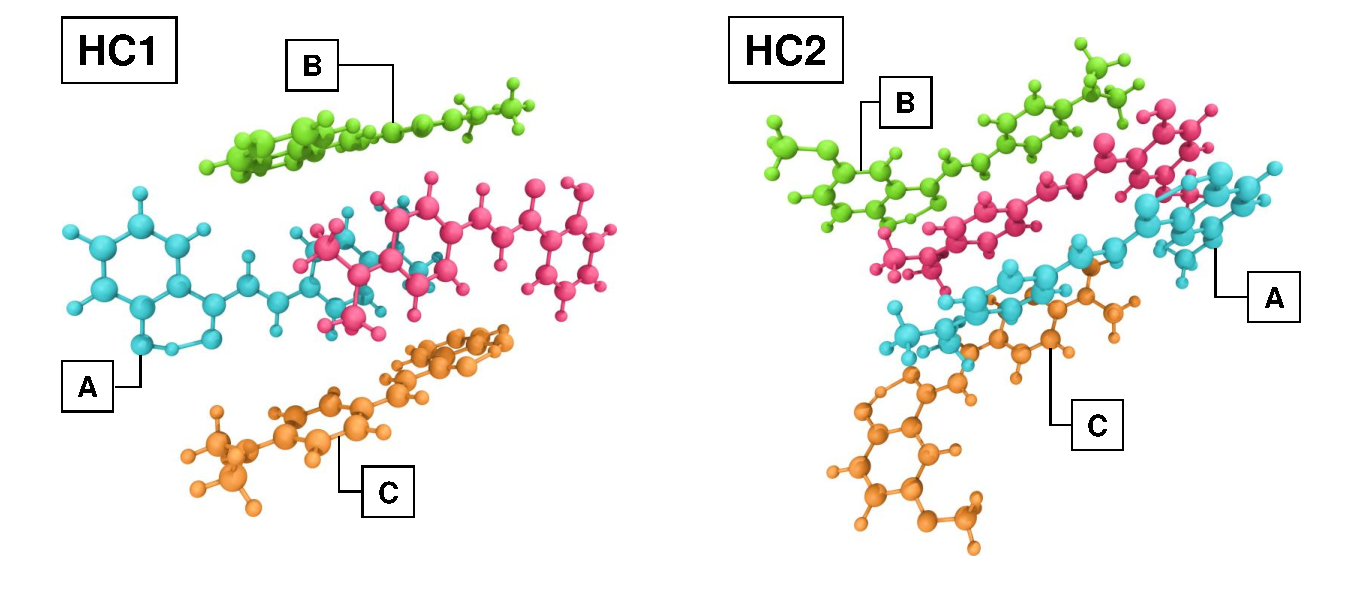
\includegraphics[width=12cm]{Chapters/5Ewald/quad.pdf}
\caption{Selected tetramer configurations from both crystals. The molecule in pink is optimised using \EEC{}.}
\label{fig:quad}
\end{figure}

\begin{figure}
\centering
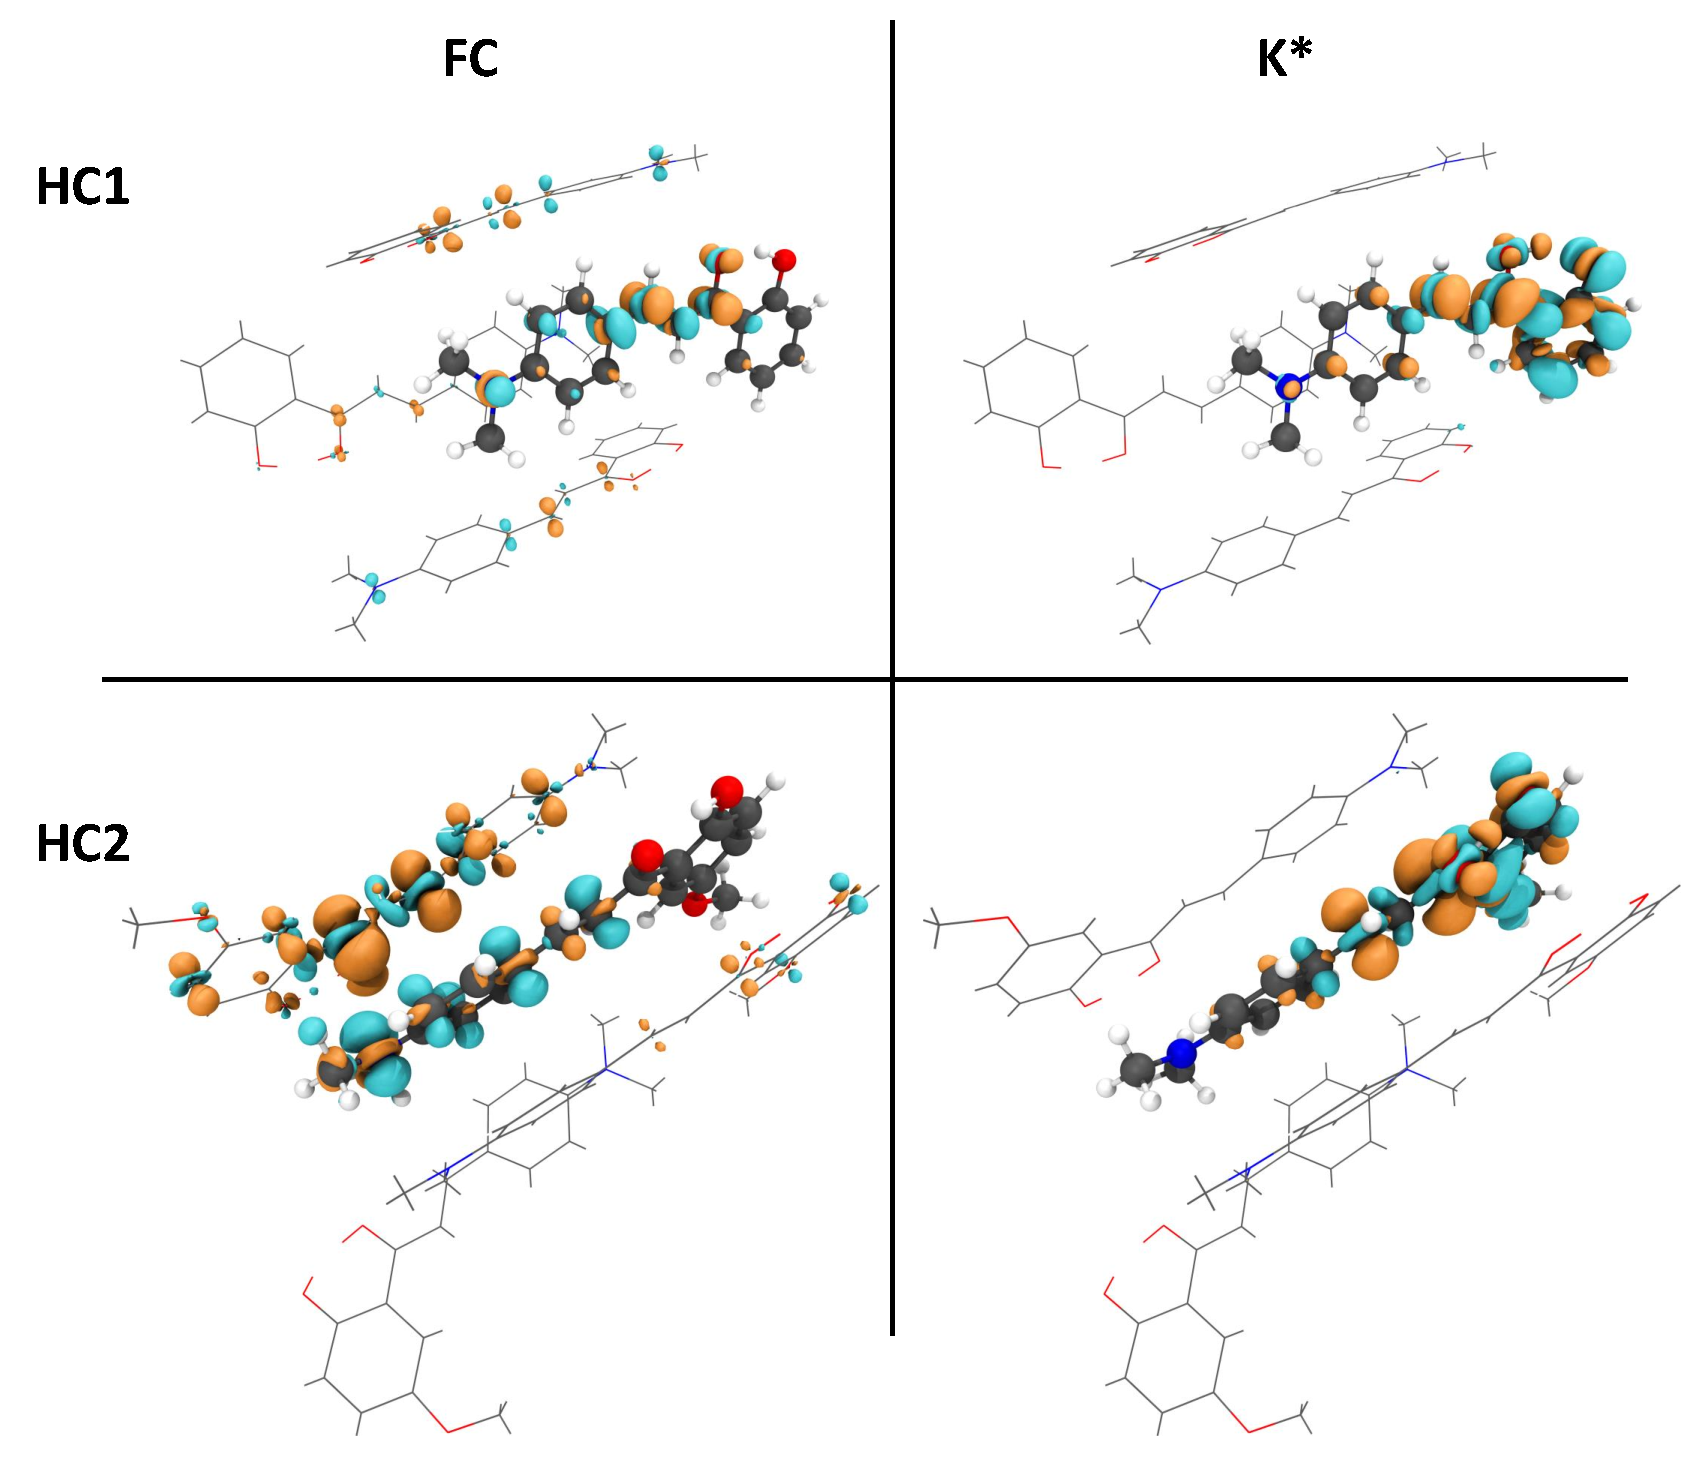
\includegraphics[width=10cm]{Chapters/5Ewald/quad_density.pdf}
\caption{S$_n$\textendash{}S$_0$ density differences obtained at TD-$\omega$B97X-D\slash{}6-311++G(d,p) level of theory for the tetramer model (excited state density gain upon excitation is shown in orange, and the loss in blue). For the \textbf{FC} geometries, the tetramer's bright states were considered ($n$=4 for \HC{} and $n$=5 for \HCC{}); for \textbf{K*}, $n$=1. All configurations were obtained by optimising the geometry of the central molecule with \EEC{}.}
\label{fig:dens}
\end{figure}


Figure \ref{fig:dens} shows the S$_n$\textendash{}S$_0$ density differences obtained for the bright state at Franck-Condon geometry (\textbf{FC}) and the \textbf{K*} S$_1$ excited state minimum geometries. The plots for the first five excited states can be found in Appendix \ref{app:sec:tetramer_vert}. When considering a full tetramer in the excited state, the bright states of \HC{} and \HCC{} are S$_4$ and S$_5$ respectively, whereas for single monomers, they are both S$_1$. An important degree of localisation is observed on monomers and dimers for both crystals, despite four molecules being included in the QM region. Consequently, we expect that with embedding charges of sufficient quality, a QM region of one or two molecules would obtain accurate excited state energies. 
  



Excitations in \HC{} are more localised than in \HCC{}, which correlates with the larger exciton couplings obtained for the latter.\cite{Dommett2017c} In the case of \HC{}, only the coupling with molecule B is larger than 0.1 eV (Appendix \ref{app:sec:tetramer_vert}). For both crystals, in the \textbf{K*} minimum, the excitation is clearly localised in the central molecule, which suggests that schemes such as \EEC{} and \SCEEC{}-S$_0$ could be best suited to describe this kind of situations (see discussion in the next sections). Additionally, the QM region with only one monomer should be able to describe emission from the \textbf{K*} form, which is confirmed by the evolution of the energies with the size of the region (see section \ref{sec:cluster}).

\subsection{Point Charge Embedding: Electrostatic Effects in the Crystal}
\label{sec:PCE}

Having now observed the localisation of the excitation upon fluorescence, we can begin assessing the performance of different embedding methods with only one monomer in the QM region. In this section, we analyse the performance of the PCE model and the effect of using different charges for the description of excited states in the \HC{} crystal. Our analysis is based on the results obtained with a monomer in the QM region. 

\begin{table}
\centering
\caption{Absorption, emission and \textbf{K-MECI} energies (in eV) of \HC{} embedded in different types of Ewald point charge arrays. Unless specified the geometries were obtained at the ONIOM(TD-$\omega$B97X-D/6-311++G(d,p):AMBER) level of theory. \textbf{K-MECI} energies are relative to the ground state energy of the Franck-Condon (\textbf{FC}) minimum.\cite{Dommett2017c} \SP{$\dagger$}Optimised geometries within the PCE environment. \SP{$\dagger$ $\dagger$}Geometry optimised in vacuum} 
\scalebox{0.9}{
\begin{tabular}{@{}>{\centering\arraybackslash}m{3cm}ccccccc@{}}

\textbf{Method} & \multicolumn{2}{c}{\textbf{Charges}} &\textbf{Absorption}  & \multicolumn{2}{c}{\textbf{Emission} } &\textbf{$\bm{S_1}$-$\bm{S_0}$}  \\ \midrule
& \textbf{Type} & \textbf{Basis} &\textbf{FC(E)}    & \textbf{E*} & \textbf{K*}    & \textbf{K-MECI}  \\ \midrule
&\multicolumn{2}{c}{\textbf{Molecular}}&\\\midrule
\multirow{7}{3cm}{TD-$\omega$B97X-D\slash{}6-311++G(d,p)}&NBO&\multirow{5}{*}{6-311++G(d,p)}&3.28 & 3.10 &2.67 & 4.35 \\
&RESP& &3.30 & 3.12 & 2.66 & 4.41 \\
&RESP (SC-PCE-S$_1$)&& 3.09 & 2.96 & 2.65 & 4.72\\
&RESP\SP{$\dagger$}&& 3.37 & - & 2.69 & 4.37 \\
&Mulliken&&1.56 & 1.51& 1.47 & 4.42 \\\cmidrule(lr){3-3}
&Mulliken& 3-21G(d)&3.29 & 3.11 & 2.70 & 4.76\\
&Mulliken& 6-31G(d)&3.35 & 3.16 & 2.70 & 4.68\\\midrule
RI-CC2\slash{}SV(P)&RESP&\multirow{2}{*}{6-311++G(d,p)}&3.11 & 2.95 & 2.35 & 3.82 \\
RI-CC2\slash{}TZVP&RESP & & 2.98 & 2.82 & 2.29 & 3.56 \\\midrule

%%&\multirow{5}{*}
&\multicolumn{2}{c}{\textbf{Crystal}}&\\\midrule
\multirow{5}{3cm}{TD-$\omega$B97X-D\slash{}6-311++G(d,p)}&RESP&\multirow{5}{*}{DZVP}& 3.33 & 3.15 & 2.68 & 4.32 \\
&AIM&  &3.35 & 3.16 & 2.68 & 4.30 \\
&Hirshfeld& & 3.43 & 3.23 & 2.68 & 4.56 \\
&Hirshfeld\SP{$\dagger$}& & 3.50 & 3.20 & 2.28 & 2.89 \\ 
&Mulliken&  &2.95 & 2.85 & 2.64 & 4.20 \\\midrule
&\multicolumn{2}{c}{\textbf{No charges}}&\\\midrule
\multirow{2}{3cm}{TD-$\omega$B97X-D\slash{}6-311++G(d,p)}& - &-&3.52 & 3.31 &2.67 & 4.76 \\
&-\SP{$\dagger$ $\dagger$}& -&3.65 & 3.28 & 0.36 & 2.84 \\\midrule 

-&Experimental\cite{Zhang2015,Zahid2017} & - &2.9, 3.3 & - &1.7\textendash{}1.9 & -\-\\\bottomrule
\end{tabular}
  }
\label{tab:point_energies}
\end{table}

The experimental absorption in the solid state shows two bands which have previously been attributed to absorption from the \textbf{E} and \textbf{K} forms.\cite{Zhang2015,Zahid2017}  Our calculations show that neither the crystal composed of \textbf{K} molecules nor the one with \textbf{K} surrounded by \textbf{E} molecules are stable in the solid state. Additionally, the experimental crystal structure does not seem to be consistent with a significant population of the \textbf{K} form in the ground state.\cite{Zahid2017} Taking this into account, the presence of \textbf{K} in the ground state seems to be associated with dynamic processes activated in the experimental conditions. For example, at room temperature, large amplitude motions of the proton along the H-bonded bridge can reduce the S$_1$\textendash{}S$_0$ energy gap to 2.76 eV, considering vibrational broadening. Additionally, given the ultrafast nature of the proton transfer in the solid state (3 ps \cite{Zahid2017}), fast absorption from \textbf{K} forms generated in the excited state could be also possible. The dynamic nature of these processes is in line with the broad structure of the low energy band. Our focus is the analysis of the higher energy band which corresponds to the absorption in the \textbf{E} form.

To estimate the effect of vibrational broadening on the position of the absorption maximum, we use the nuclear ensemble method\cite{Crespo-Otero2012a} as implemented in \texttt{Newton-X}\cite{newtonx} with TD-$\omega$B97X-D/6-311++G(d,p) embedded in RESP charges. In this method, a normal mode calculation of the molecule is carried out in the ground state. Geometries are then sampled from these normal modes using a Wigner distribution, and vertical absorptions are calculated at each sampled point. The position of the \textbf{E} absorption maximum (3.21 eV, 0.1 eV shift with respect to the vertical excitation with the same method) is in excellent agreement with the experimental value (Appendix \ref{app:sec:spectra}). 

To directly evaluate the effect of charges of different origin, we compare absorption, emission (from \textbf{E*} and \textbf{K*} forms), and S$_1$\textendash{}S$_0$ MECI energies with Ewald embedding. Given that the MECI associated with the enol pathway was consistently found to be at least 4 eV higher in energy than its keto counterpart, we will focus on the \textbf{K-MECI} deactivation pathway. The results are summarised in Table \ref{tab:point_energies}. In order to directly compare the impact of different charge partition schemes, we use the same geometry throughout, obtained at the ONIOM(TD-$\omega$B97X-D/6-311++G(d,p):AMBER) level of theory.\cite{Dommett2017c}. 


Excited state calculations with PCE using non-Mulliken charges predict the maximum of absorption with close agreement to the experimental value of 3.3 eV. Overall, the effect of the embedding is to shift absorption to the red with respect to the energy obtained in vacuum (3.65 eV). For calculations at fixed geometries, there is no significant dependence on whether the charges are obtained from molecular or crystal calculations. In particular, the energies obtained using RESP charges are consistent between the molecular and the crystal descriptions. In the context of the molecular organic crystals, this is not surprising as RESP charges are designed to match the electrostatic potential, and crystal packing has but a small effect on the electronic structure of these molecules due to their non-bonded nature.

In contrast, calculations using Mulliken charges strongly depend on the choice of basis set (both the size and the type). With these charges, results with smaller basis sets are closer to the experimental value. They provide reasonable energies with 3-21G(p) and 6-31G(d), but fail to reproduce sensible values if a larger basis set is used (6-311++G(d,p)). This is in line with the well-known sensitivity of the Mulliken method to the basis set.


The experimental emission in the solid state has been attributed to the \textbf{K*} form.\cite{Dommett2017c} Regardless of the higher stability of \textbf{K*} in the excited state, emission from the \textbf{E*} form is expected to be close to the initial absorption and consequently reabsorbed. Accordingly, our TDDFT calculations predict emission from \textbf{E*} in the range of 3.1\textendash{}3.3 eV. Interestingly, emission from the \textbf{K*} form ({\raise.17ex\hbox{$\scriptstyle\sim$}}2.7 eV) is significantly deviated from the experimental values (1.7\textendash{}1.9 eV).\cite{Zhang2015,Zahid2017} This is not improved by using self-consistent point charges in the SC-PCE-S$_1$ method, which is to be expected due to the localisation of the excited state to one molecule (Figure \ref{fig:dens}). When the emission is calculated using RI-CC2, the energy is improved but is still deviated by more than 0.5 eV from the experiments. 

The most significant factor is the geometry itself, obtained at QM:MM level. We show later that a better emission energy is obtained when optimisation is done using the \EEC{} and \SCEEC{} methods. When it comes to the optimisation of excited state minima and S$_1$\textendash{}S$_0$ MECI, the PCE approach was unsuccessful in locating stable minima for most charges types, due to the lack of non-Coulombic short-range interactions and ensuing overpolarisation effects. Only Hirshfeld and, in certain cases, crystal RESP charges were overall small enough in magnitude to allow for the determination of local minima, with the largest charge on an atom od 0.5 e$^-$. As such optimisation with PCE in general is not recommended for systems with a high degree of conformational flexibility.

As for S$_1$\textendash{}S$_0$ MECI energies, all TDDFT results for the QM:MM geometries are more than 1 eV above the \textbf{FC} bright state energy (Table \ref{tab:point_energies}). The conical intersections are thus rendered inaccessible as expected since \HC{} displays aggregation-induced emission. The energies obtained with RI-CC2 are in the range of 0.6\textendash{}0.7 eV above their corresponding excitation energies which also makes them inaccessible. These results are consistent within the RACI model but are overestimated with respect to the value of 3.97 eV obtained with QM:MM with a dimer in the QM region.\cite{Dommett2017c}

In the case of RESP charges, optimisation within the PCE model does not significantly change the energetics previously evaluated with single point calculations. Indeed the structures are close to those reported at the QM:MM level of theory. The resulting relative energies are shown in Figure \ref{fig:pts_n_vac}. For Hirshfeld charges, the effect of optimisation is more significant reducing the \textbf{K*} emission energies to 2.28 eV and making the S$_1$\textendash{}S$_0$ MECI accessible.


\begin{figure}
\centering
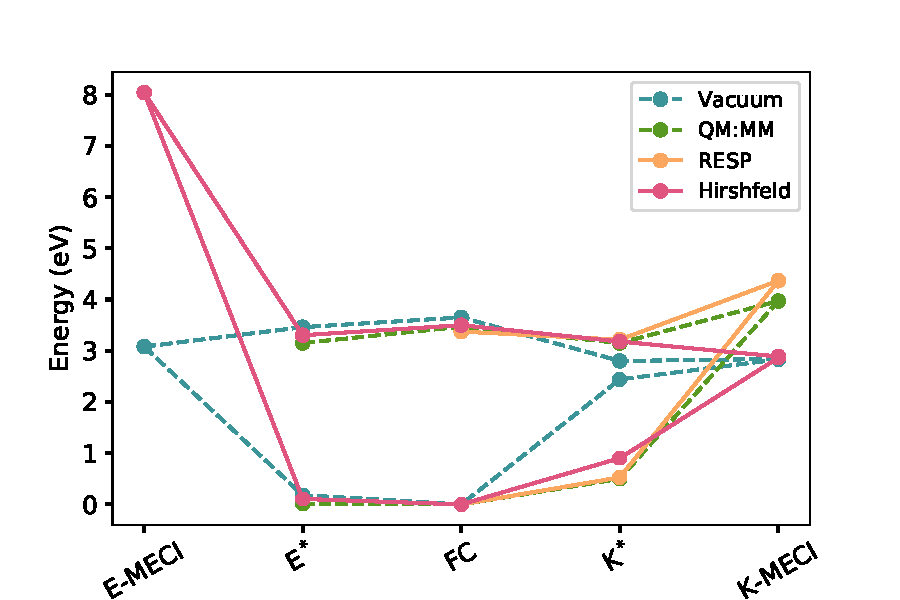
\includegraphics[width=9cm]{Chapters/5Ewald/Energies_Figure.pdf}
\caption{Energies \HC{} in vacuum and embedded in RESP and crystal Hirshfeld Ewald charges at different geometries. QM:MM energies were taken from Ref \citenum{Dommett2017c}.}
\label{fig:pts_n_vac}
\end{figure}

Comparing the calculations in PCE and vacuum at the same geometry highlights the main effects of the crystal electrostatic environment in the excited state. The excited states are overall stabilised which reduces both the vertical excitation and conical intersection energies. However the accessibility of the latter depends on the former, netting no clear difference in emissive behaviour. A more substantial relative stabilisation of the MECI is observable when the molecule is fully optimised in vacuum. It reaches a highly distorted geometry which would be inaccessible in the solid due to short-range interactions of the closely packed neighbouring molecules.

Our simulations show some of the drawbacks of the PCE method, in particular for its use in geometry optimisation. Because of the effects of overpolarisation and the lack of short-range non-Coulombic interactions, electrostatic forces can become too large and some nuclear configurations become unstable. Consequently, we do not recommend the use of PCE for geometry optimisations. While the method is effective in some cases,\cite{Wilbraham2015,Presti2017} it is unpredictable whether it will provide reliable geometries for all regions of the PES. To mitigate these problems we implemented a two level embedded cluster model.


\subsection{Embedded Cluster Models: Potential Energy Surfaces in the Crystal}
\label{sec:cluster}

We obtained the geometries of notable regions of the PES for \HC{} and \HCC{} crystals using the \EEC{} and its self-consistent variant \SCEEC{} methods. Table \ref{tab:em_abs} shows the absorption and emission energies obtained after optimisation of \textbf{FC} and \textbf{K*} forms using these models.  

\begin{table}[H]
\centering
\caption{Table of absorption and emission energies for both model systems after geometry optimisation with cluster models. The level of theory was TD-$\omega$B97X-D\slash{}6-311++G(d,p). Energies are in eV.\SP {$\dagger$}Charges obtained for the \textbf{K*} form in S$_1$}
\label{tab:em_abs}
\begin{tabular}{@{}ccccc@{}}


\toprule
\multirow{2}{*}{\textbf{Cluster model}}& \multicolumn{2}{c}{\HC{}}                 & \multicolumn{2}{c}{\HCC{}}   \\ \cmidrule(lr){2-3} \cmidrule(lr){4-5}
 & \multicolumn{1}{c}{\textbf{FC}}               & \multicolumn{1}{c}{\textbf{K*}}           & \multicolumn{1}{c}{\textbf{FC}}          & \multicolumn{1}{c}{\textbf{K*}}              \\ \midrule
\EEC{}
& 3.37 & 2.06 & 3.41 & 2.07 \\

\SCEEC{}-S$_1$
& 3.08 & 2.60 (2.12)\SP{$\dagger$} & 3.34 & 2.15 \\

%\SCEEC{} \textbf{K*} S$_1$
%& - & 2.18 & - & -\\

\SCEEC{}-S$_0$
& 3.27 & 2.19 & 3.40 & 2.07 \\ \midrule

\EC{}
& 3.27 & 2.40 & 3.42 & 2.03 \\

PCM
& 3.32 & 2.36 & 3.72 & 2.44 \\ 
SC-PCM
& 3.00 & 2.66 & 3.01 & 2.21 \\
ONIOM QM:MM (molecule)\cite{Dommett2017c}
& 3.32 & 2.72 & 3.50 & 2.17 \\ 
ONIOM QM:MM (dimer) \cite{Dommett2017c}
& 3.27 & 2.61 & 3.29 & 2.19 \\\midrule\midrule
Experimental\cite{Zhang2015,Zahid2017}
& 2.9,3.3         & 1.7 - 1.9     &  -    & 1.8       \\ \bottomrule
\end{tabular}
%}\par
%\end{adjustwidth}
\end{table}

 Geometry optimisation using the embedded cluster method produces ground state geometries very similar geometries to QM:MM, consequently the absorption energies are not significantly altered between PCE (Table \ref{tab:point_energies}) and \EEC{} or SC-PCE-S$_1$ and \SCEEC{}-S$_1$ provided that RESP charges are used throughout (Table \ref{tab:point_energies}). For comparison, we have added the results obtained with ONIOM (QM:MM) including one and two molecules in the QM region and with the \EC{} model. Moreover, we present results in PCM and its self-consistent variant, both in DCM solvent, since continuum models are a common method employed to reflect the electrostatic environment in molecular condensed matter.\cite{Skelton2015} 

For all cluster models, the effect of the polarised response of the environment is to reduce the vertical excitation. This is also observed in the comparison between the PCM and SC-PCM models and when the size of the QM region increases from a molecule to dimer. The results obtained with the \SCEEC{} procedure depend on the level of excitation in the self-consistent loop. If ground state charges are used, as expected, the energies are similar to those obtained with \EEC{} (3.27 and 3.37 eV for \HC{} and 3.40 and 3.41 for \HCC{}). The emission energies obtained with different methods strongly depend on the rotation angle (Figure \ref{fig:molecules}). In vacuum, the excited state minima show a significant deviation from their ground state planar structure. In the solid state, the \textbf{K*} geometries obtained with QM:MM and \SCEEC{}-S$_1$ are more planar (\HC{}: $6 \degree$ and $9 \degree$, \HCC{}: $16 \degree$ and $12 \degree$ respectively for the angle depicted in Figure \ref{fig:molecules}) than those obtained with \EEC{} (\HC{}: $32 \degree$, \HCC{}: $18 \degree$).





%{\bf

The optimisation of the \textbf{K*} form with the OEEC model significantly improves the emission energies with respect to those obtained using QM:MM geometries. Figure \ref{fig:error} summarises the deviation of the calculated emission energies with respect to the experimental data.

\begin{figure}
\centering
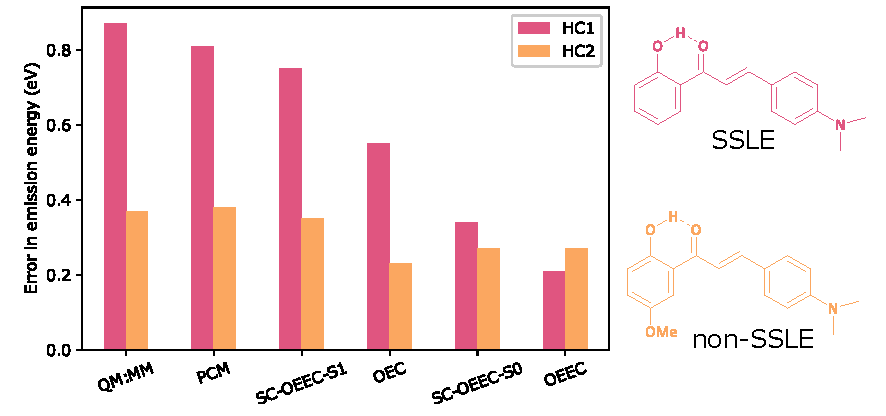
\includegraphics[width=9cm]{Chapters/5Ewald/scheme.pdf}
\caption{Deviation of the predicted emission energies of \HC{} and \HCC{} with respect the experimental values by different embedding models. Reference experimental values were 1.8 eV for both \HC{} and \HCC{} crystals}
\label{fig:error}
\end{figure}

For \HC{}, the result is 2.06 eV (TD-$\omega$B97X-D\slash{}6-311++G(d,p)), which is in close agreement with the experimental value. As with the PCE method, the self-consistent background based on the excited state charges at the \textbf{FC} state does not improve the results (2.6 eV). If ground state \textbf{E} charges are employed in the self-consistent loop, the emission energies remain in better agreement with the experimental values. Indeed, given the level of localisation of the excitation in these systems (Figure \ref{fig:dens}), the use of ground state charges seems to be more appropriate (\SCEEC{}-S$_0$) with emission energy of 2.19 eV. An alternate version of \SCEEC{}-S$_1$ is also employed where the self-consistent loop is carried out on a molecule in its \EEC{} optimised \textbf{K*} geometry, which brings the emission energy to 2.12 eV. However, this charge background represents the situation where all molecules in the crystal exhibit charges from the keto form, which we have not found to be a stable minimum in the crystal.



Comparison of the \EEC{} with the \EC{} model indicates that long-range interactions account for more than 0.3 eV in the \textbf{K*} emission energy of \HC{}.  Interestingly, while the energies for \HC{} strongly depend on the charge background, the values for \HCC{} are less affected. In the case of \HCC{}, \SCEEC{}, \EEC{} and \EC{} all provided very similar results (2.15, 2.07 and 2.07 eV), suggesting that the most important Coulomb effects are recovered at the short-range. This is linked to the difference between the ground and excited state charges of these molecules. For \HC{}, excitation significantly alters the charges of carbon atoms in the bridge, since it concentrates a large fraction of the molecule's $\pi$ orbitals (Appendix \ref{app:sec:pop_analysis_aggregates}). In the case of \HCC{} only the charge of the carbonyl carbon (C$_k$) changes more than 0.1 $e^-$ upon excitation, since the electronic reorganisation is concentrated in the back ring (Figure \ref{fig:dens}). Consequently, the S$_1$-S$_0$ energy gaps for \HC{} are far more dependent on the electrostatic environment. Indeed improving the description of the short-range intermolecular interactions does not significantly alter the energy gaps, as illustrated by the behaviour of the absorption and emission energies with the size of the QM region (see end of section). For both, \HC{} and \HCC{}, the emission from \textbf{K*} is fairly well reproduced with only one molecule in the QM region, which is in line with the localised nature of the \textbf{K*} (Figure \ref{fig:dens}).



Conical intersections play a key role in photophenomena, providing a radiationless decay funnel for the excited state. One of the features implemented in \texttt{fromage} is the searching of crossing geometries using the penalty function method of Levine \textit{et al.}\cite{Levine2008} The molecules considered here can deactivate to the ground state in solution via conical intersections associated with intramolecular rotation.\cite{Dommett2017a,Dommett2017c} We optimise  the S$_1$\textendash{}S$_0$ MECI with the SA-2-CASSCF(12,11)/6-31G(d) and TD-$\omega$B97X-D\slash{}6-311++G(d,p) methods within the \EEC{} scheme (Figure \ref{fig:ci}). For these systems, the geometries obtained with both levels of theory are in very good agreement. 



\begin{figure}
\centering
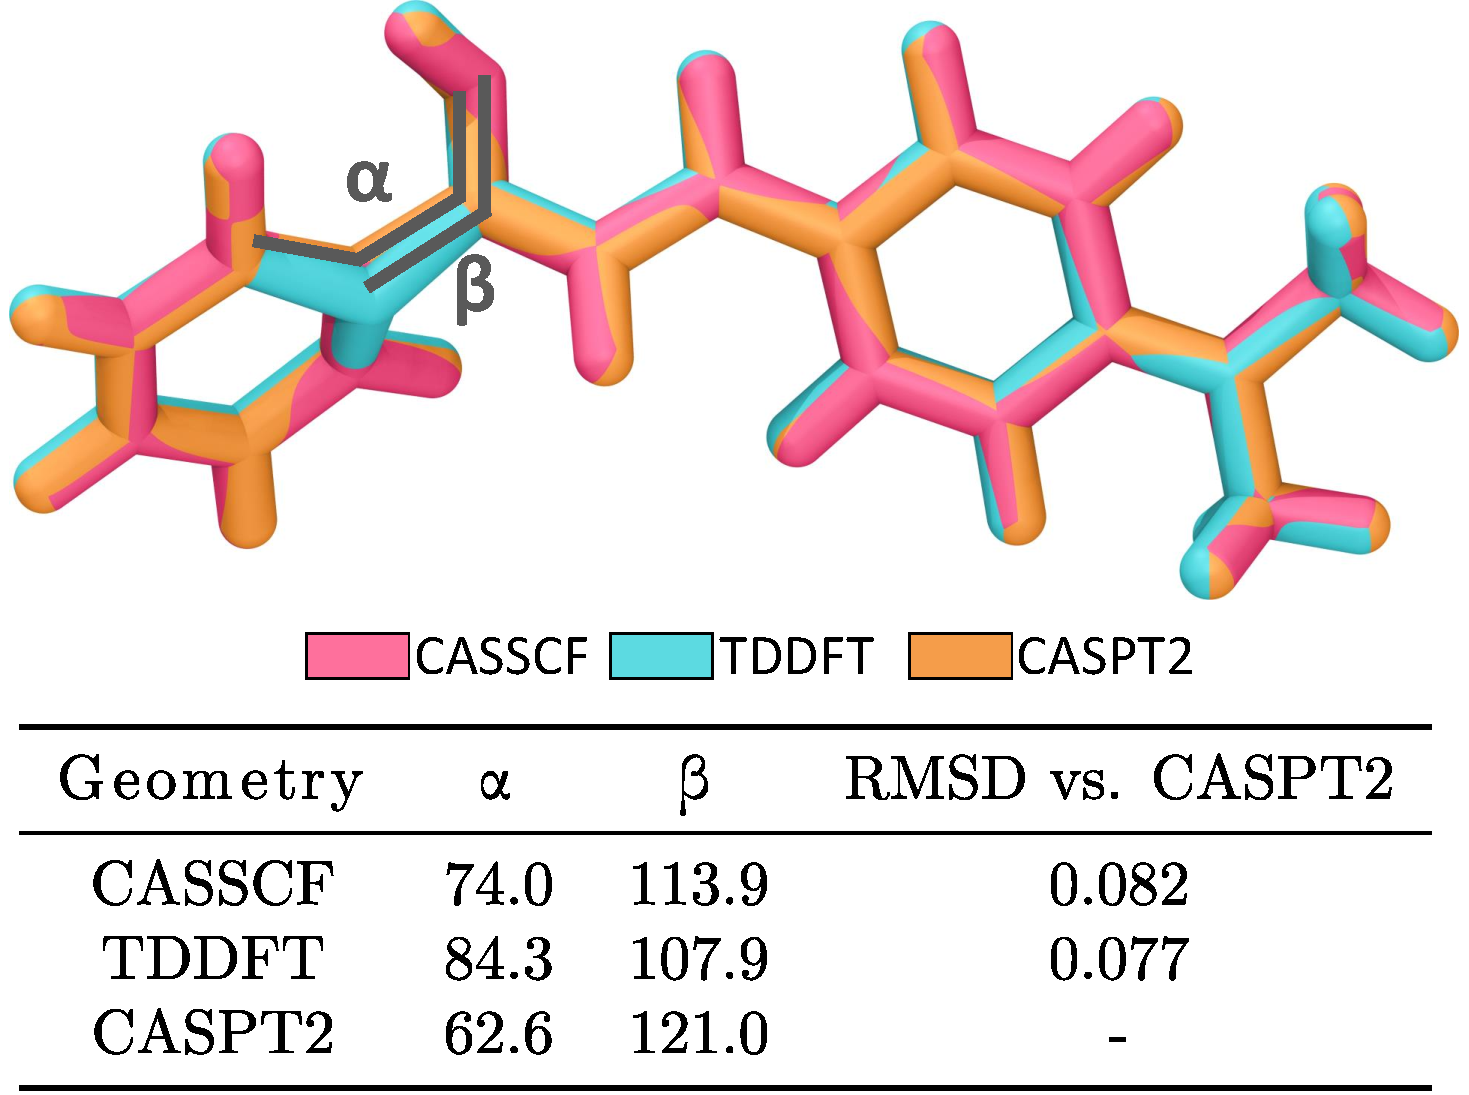
\includegraphics[width=8cm]{Chapters/5Ewald/ci_fig.pdf}
\caption{MECI geometries found with SA-2-CASSCF(12,11)/6-31G(d) and TD-$\omega$B97X-D\slash{}6-311++G(d,p). Additionally, we include the configuration with least S$_1$\textendash{}S$_0$ gap when scanning the $\beta$ angle from the TDDFT geometry at MS-2-CASPT2(12,11)/6-31G(d) level. It is labelled CASPT2.}
\label{fig:ci}
\end{figure}

In the crystal, the lowest energy conical intersection combines intramolecular rotation and a significant pyramidalisation of the carbonyl carbon.\cite{Dommett2017c} In the gas phase, the lowest energy conical intersection only involves intramolecular rotation while the one also involving pyramidalisation is higher in energy. Therefore one of the effects of the crystal environment is to modify the stability of the lowest energy conical intersections, which is consistent with the results obtained with QM:MM calculations. This confirms that the effect of short-range interaction is essential in determining the geometry while the long-range interactions modulate the total energy. However, the net effect of the embedding on the total energies is highly system dependent. 

 
 \begin{figure}
\centering
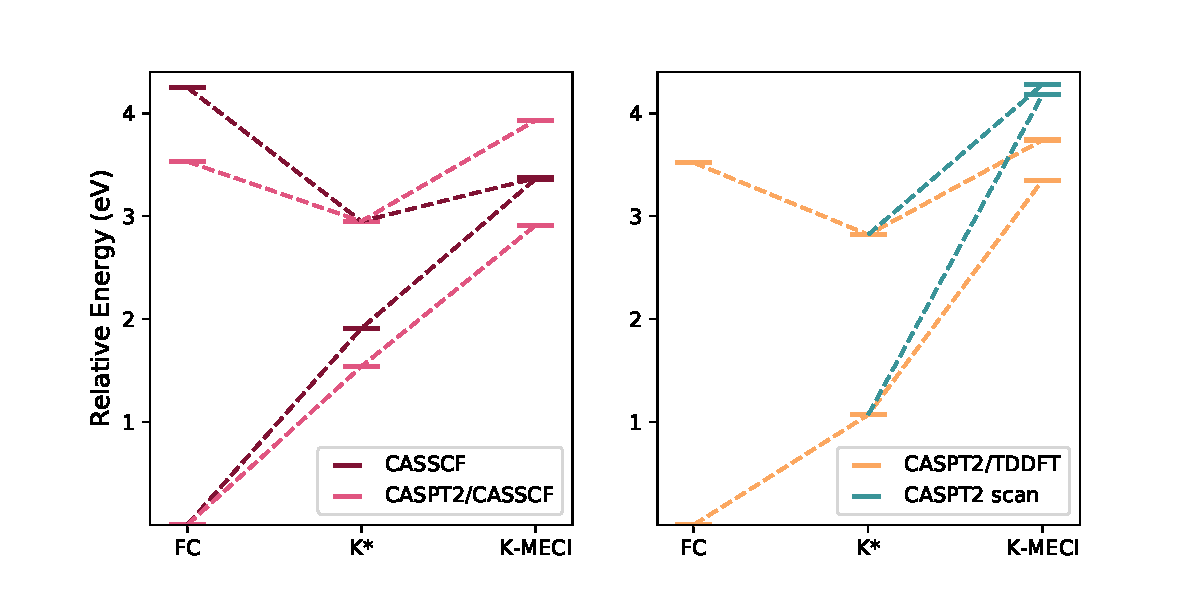
\includegraphics[width=12cm]{Chapters/5Ewald/CAS_energy_figs.pdf}
\caption{Relative energy diagrams showing the emission energy and accessibility of the MECI with multireference methods at the geometries shown in Figure \ref{fig:ci}. To minimise the CASPT2 S$_1$\textendash{}S$_0$ gap at MECI configurations, a geometry scan was carried out as described in Figure \ref{fig:scan}. The newly optimised geometry is labelled ``CASPT2 scan'' and has a gap of 0.10 eV.}
\label{fig:ci_ener}
\end{figure}

Figure \ref{fig:ci_ener} shows the PES obtained with multireference methods.  The  vertical excitation obtained with SA-2-CASSCF(12,11)/6-31G(d) is significantly deviated from the experimental value (4.25 eV compared to 3.3 eV). Including dynamic electron correlation with MS-2-CASPT2(12,11)/6-31G(d) shifted the value to the red in much better agreement (3.53 eV). The energy gap at the CASSCF conical intersection is too large with PT2 (1.02 eV), but using TDDFT geometries as reference can significantly narrow the gap. These are common challenges found in multireference calculations and not due to the embedding approach.\cite{Peng2016,Crespo-otero2017,Barbatti2012} In order to further narrow the S$_1$\textendash{}S$_0$ gap, the aromatic C was systematically displaced \textit{via} the $\beta$ angle (Figure \ref{fig:ci}). Figure \ref{fig:scan} shows how this scan locates a conical intersection at an energy 0.8 eV above the \textbf{FC} energy. These examples show that the Ewald embedding methods can provide all the information required to fully characterise the PES in molecular crystals. All of these methods are available in \texttt{fromage}. 

 
\begin{figure}
\centering
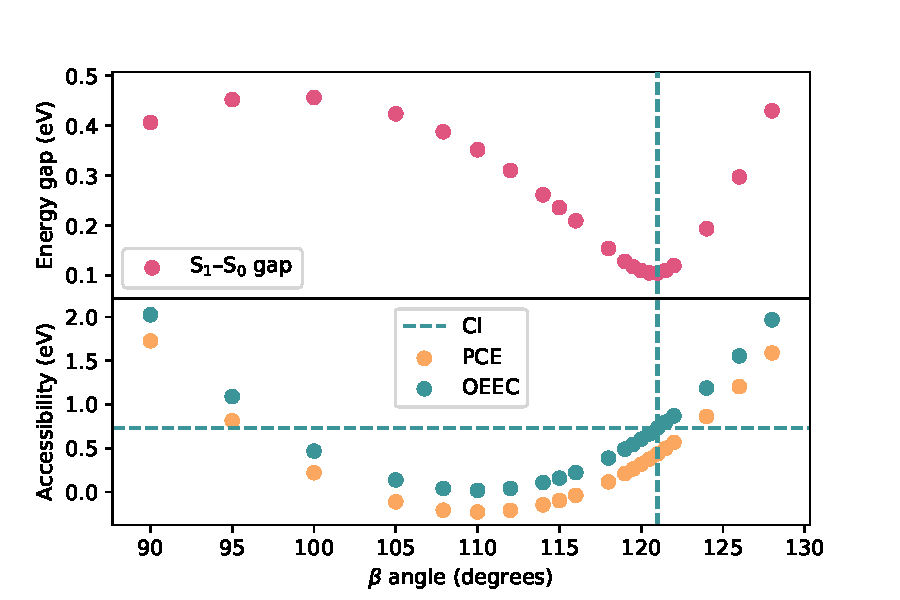
\includegraphics[width=9cm]{Chapters/5Ewald/energy_scan.pdf}
\caption{Plot of the S$_1$\textendash{}S$_0$ gap, and the MECI accessibility as a function of the puckering angle $\beta$. The accessibility is defined as the average S$_1$\textendash{}S$_0$ energy of the given geometry minus the \textbf{FC} bright state energy. The \EEC{} energy at the geometry with smallest S$_1$\textendash{}S$_0$ gap is indicated by dashed lines.}
\label{fig:scan}
\end{figure}

Given that the Ewald embedding methods describe the effect of the electrostatics of the whole crystal, they represent unique schemes to analyse the convergence of properties with the size of the QM region. Exploring these effects is essential in systems with significant excitonic effects. We consider the behaviour of the energies and the accessibility of the S$_1$\textendash{}S$_0$ MECI with the size of the QM region (Figure \ref{fig:cluster}). We employ the TD-$\omega$B97X-D\//6-31G(d) level of theory, which provides a good description of different regions of the PES. For \HC{}, the energies of the bright state for \textbf{FC} and of the emission from \textbf{K*} converge relatively quickly. On the other hand, the energy of the S$_1$\textendash{}S$_0$ MECI increases with the size of the QM region for \HC{} and decreases for \HCC{} respectively becoming less and more accessible. This is in line with the experimental behaviour of both crystals.



\begin{figure}
\centering
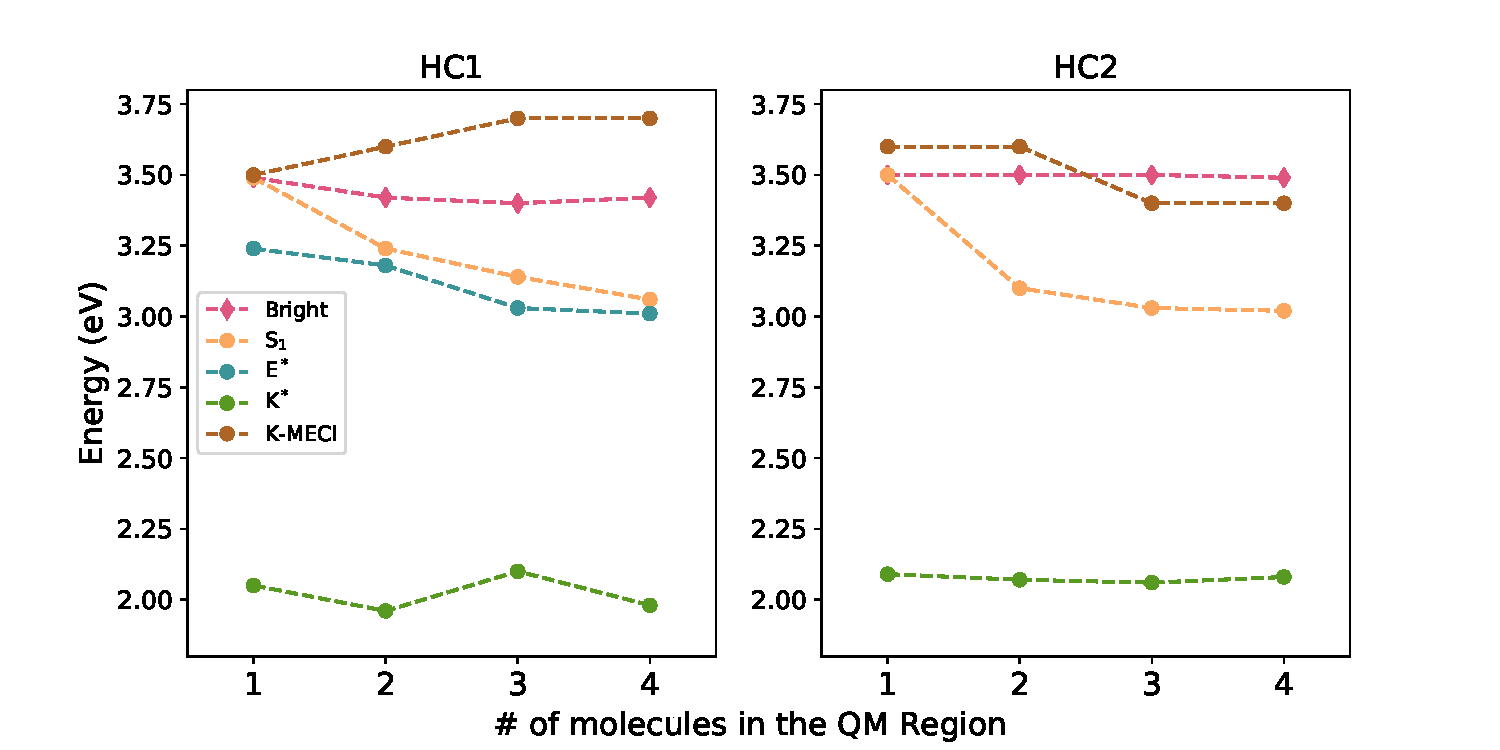
\includegraphics[width=12cm]{Chapters/5Ewald/aggregates.pdf}
\caption{Energy of the absorption, emission and conical intersection as the excited state region increases in size using the \EEC{} model. The region molecules are added to the region in the order displayed in Figure \ref{fig:quad}. The energies are evaluated with TD-$\omega$B97X-D\slash{}6-31G(d).}
\label{fig:cluster}
\end{figure}


\section{Conclusion}

In this chapter, we analysed the behaviour of different Ewald embedding schemes for the description of excited states in molecular crystals. With focus on the exploration of potential energy surfaces, we have implemented these methods in the Python open-source platform \texttt{fromage}, which we make readily available.  This program enables users to easily combine electronic structure codes of their choice for geometry optimisation using \EC{}, \EEC{} and \SCEEC{}. The current implementation includes interfaces to popular quantum chemistry programs such as \texttt{DFTB+}, \texttt{Turbomole}, \texttt{Gaussian} and \texttt{Molcas}. Additional interfaces can be easily implemented, provided that the new codes allow for gradient calculations with point charge embedding.

We have shown that the PCE method is poorly suited to optimising the geometry of flexible molecules in the crystal form. Consequently, the photochemical conclusions that arise from PCE calculations of such molecules have the potential to be quantitatively and qualitatively erroneous. To overcome this problem, a series of two-level ONIOM(QM:QM') cluster models with Ewald embedding were formulated. They are suitable for geometry optimisation of excited state minima and conical intersections, and include long range electrostatic system-environment interactions within the crystal, thus addressing the fault in traditional cluster models outlined in Section \ref{sec:prob_lr}.

The potential of these tools was illustrated by applying them to the excited states of two model crystals, \HC{} and \HCC{}, displaying excited state intramolecular proton transfer. \HC{} displays aggregation induced emission whilst \HCC{} shows no emission in solution or solid state. For both systems, the excitations are clearly localised in one or two molecules which allowed the emission energies to converge with only a monomer or a dimer in the QM region. We found that using charges originating from molecular or crystal calculations did not significantly impact the results. The emission energy was progressively improved with a hierarchy of embedding models, ranging from a deviation from the experimental emission peak of 0.8 eV with ONIOM QM:MM to 0.2 eV with \EEC{}. Due to the flexibility of the molecules, this increase in accuracy could only be achieved by carrying out geometry optimisation with each embedding model.  
 
 Self-consistent procedures help to model the mutual polarisation between the excited state region and the environment, a known problem of ONIOM models presented in Section \ref{sec:prob_sc}. In particular, if the self-consistent loop is carried out in the excited state, these procedures may help reflect the delocalisation of an excitation despite explicitly modelling fewer excited fragments than are involved in the delocalisation. For the systems considered in this study, the degree of localisation in both the absorption and emission processes made excited state self-consistent embedding unsuitable. The application of the self-consistent procedure to the ground state did not significantly alter the results obtained from the corresponding non-self-consistent procedure which suggests that the electronic structure of the isolated ground state molecule is not particularly altered by crystal packing. 
 
 With these conclusions in mind, we can suggest optimal embedding methods for the study of the photochemistry of different molecular crystals. If the molecule is certain to be structurally rigid and the exciton couplings are small, the PCE scheme can be appropriate. Otherwise, cluster models are preferred since they allow for exploration of the nuclear configuration space. In either case, long range electrostatic interactions can account for a significant contribution to the excited state energy. Comparison between excitation energies obtain with truncated cluster models and single point calculations with Ewald embedding methods can help decide whether these methods are required.  
 
 The size of the QM region should be motivated by the locality of the excitation at the noteworthy points of the PES which can be estimated by the calculation of exciton couplings between molecular fragments in their lattice positions. These coupling values can, in turn, be estimated as half of the S$_2$\textendash{}S$_1$ energy gap for the dimer\cite{Spano2016} or by using more sophisticated methods (see Section \ref{sec:detail_js}). For localised excitations, ground state background charges can be a good choice (either \EEC{} or \SCEEC{}-S$_0$). If the excitation is delocalised and the QM region becomes impractically large, the \SCEEC{}-S$_1$ method can provide a better description of the excited states. We believe the use of these methods will contribute to a better understanding of complex photochemical processes in the crystal environment, impacting a broad range of applications. 
